\documentclass[a4paper]{article}
\usepackage[swedish, english]{babel}
\usepackage[T1]{fontenc}
\usepackage[sectionbib, round, authoryear, longnamesfirst]{natbib}
\renewcommand{\rmdefault}{pad}
\usepackage{graphicx}
\usepackage{tabularx}
\usepackage[a4paper]{geometry}
\usepackage{url}
\usepackage{amsmath}
\numberwithin{equation}{section}
\usepackage{makeidx}
\makeindex

% Different font in captions
\newcommand{\captionfonts}{\footnotesize}
\makeatletter  % Allow the use of @ in command names
\long\def\@makecaption#1#2{%
  \vskip\abovecaptionskip
  \sbox\@tempboxa{{\captionfonts #1: #2}}%
  \ifdim \wd\@tempboxa >\hsize
    {\captionfonts #1: #2\par}
  \else
    \hbox to\hsize{\hfil\box\@tempboxa\hfil}%
  \fi
  \vskip\belowcaptionskip}
\makeatother   % Cancel the effect of \makeatletter

\renewcommand{\figurename}{Fig.}

\title{Music, Computers and Interaction\\Collected papers}
\author{Henrik Frisk\\henrik.frisk@mhm.lu.se\\Malm� Academy of Music,
  Lund University}

\begin{document}
\selectlanguage{english}

 \chapter{New communications technology in the context of interactive sound art: An empirical analysis}
 \label{cha:new-comm-tech}

\section{Epigraph}
\label{sec:epigraph}

This essay was originally published in \emph{Organised Sound} in 2005. A revised version of it appeared in Miya Yoshida's
PhD dissertation \emph{The Invisible Landscapes: The construction of new subjectivities in the era of the mobile telephone} (2006) \citep{frisk05,yoshida06}

\begin{abstract}
  In this article we discuss the notion of `interaction' and
  `participation' and `the public' in artistic work, specifically
  within the context of the exhibition The Invisible Landscapes
  (curated by Miya Yoshida, Malm\"{o} Konstmuseum, 2003) and
  etherSound (created by Henrik Frisk), a sound installation displayed
  in that exhibition. In this work the audience is invited to
  participate in the creation of new sound events by sending text
  messages from their mobile phones. Thus, our discussion is focused
  on the space and the mode of participation opened up by new
  communication technology. Based on our experiences of that project,
  we introduce and explain what we believe are relations of creative
  production and a different kind of creativity that may emerge from
  active interaction. We also attempt to describe what we believe an
  implementation of active public participation can lead to.

  We are combining two modes of thinking in this article - one is
  inspired by discourse of the cultural theories and the other is the
  reflection upon our experience of the event. The latter is by
  definition rather subject-centered and expansive based on individual
  observation. We examine and analyze the phenomenon of
  `participation' whilst playing \emph{etherSound} as a process of creative
  production, and seek to reflect upon the power of the co-operative
  practice and its relation to participation and creativity.
\end{abstract}

%%% Local Variables: 
%%% mode: latex
%%% TeX-master: "../stim_create"
%%% End: 

% \epigraphhead[0]{
% \epigraph{The first version of this article was presented at the
%   \emph{Spark Festival of Electronic Music and Art} in Minneapolis,
%   USA in 2005 and appeared in print in the program book for the
%   festival. The article has been revised and edited for this
%   context.}{\citep{frisk1}}}
% \begin{minipage}[t]{0.6\linewidth}
%   \begin{large}
%     \textbf{Author:} \emph{Henrik Frisk}
%   \end{large}
% \end{minipage}


\section{Introduction}
The\footnote{Frisk \& Yoshida, New Communications Technology in the Context of Interactive Sound Art: an empirical analysis, \emph{Organised Sound} 10:2, 121-7, 2005, \copyright~Cambridge
University Press, reproduced with permission.} notion of `participation' has been widely discussed in the context
of contemporary culture. In the visual arts Marcel Duchamp opened up
the space as an `art coefficient'\footcite{bourriaud} and the happenings
and performances in the Fluxus movement were theorized as spectator
`participation'. In the late 70's a strong critique of the cultural
institutions originated in the United States and Europe. There was
still a strong connection between social class and arts consumption
\footcite[See for example][]{dimaggio, bourdieu}. As the question of authenticity occurs in
the 80's, and the concept of site specificity comes into focus, it
influences the attempts to broaden the audiences. In the 90's, the
emergence of a new public art and a trend of `Relational Art'\footcite{bourriaud}, such as social service and banal daily events; and
community-based art, made `participation' a central issue for cultural
production. The art activities, shortly described above, strongly
suggests diverse interpretations of the notion of 'participation' and
the necessity for constant reinterpretation of the term. What does
`participation' mean in the age of the Internet and mobility? Who can
be conceived of as a participant? What does the factor of
`participation' produce?

With the popularity of communication technology and mobility, the
definition of contemporary culture is transforming. Bataille conceived
that a definition of culture is deeply related to the way society
chooses to annihilate excess energy\footcite{bataille}. Applying his
words to the networked society, the surplus is observed in the
phenomena of the excess volume of communication through new media,
which eventually produces a new space. Furthermore, we can look at
communication as a potential area for the emergence of a new culture
that differs from the pre-existing categories and class hierarchies.
Instead of an inherited cultural capacity in society, the flow of
communication strongly impacts the cultural sphere and mutates the
recipients and stimulates the creative capacity. Although in large,
much of the need for communication and the need for new tools for
communication is created by economical interests, we argue that
communication in a certain sense and under certain conditions can be
considered as a new production of culture.

\begin{figure}[!ht]
  \begin{center}
    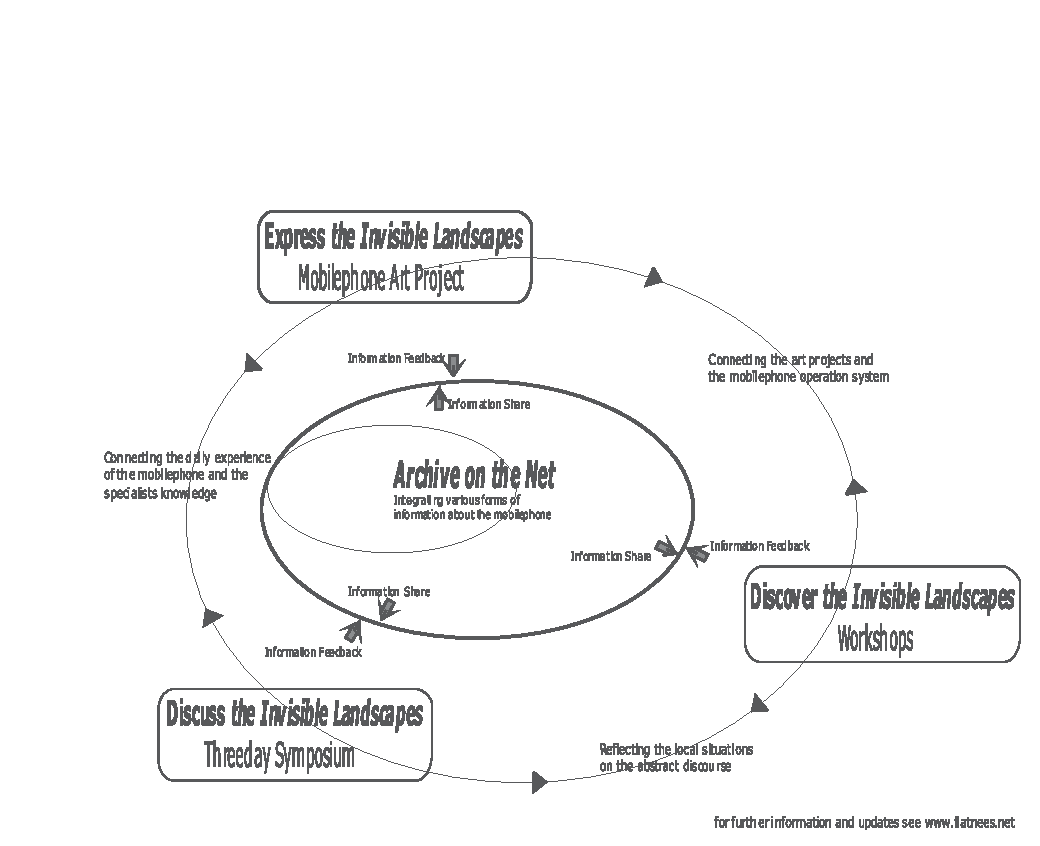
\includegraphics[width=\linewidth]{img/InvLandscape}
    \caption{Map of events for the project \emph{The Invisible Landscapes}.}
  \end{center}
\end{figure}
% \movetoevenpage

% This is a comment to the section collaborative music.

% \cleartorecto

\section{Collaborative music}
Collaborative musical compositions and sound art has been realized in
a number of ways and with different objectives. In the project
\emph{Norge - et lydrike, Norway Remixed} the curatorial idea was `to
bring the whole country together through sound', so `the local branch
offices of the broadcasting corporation' was supplying sound material
`in order to secure authenticity' and `actively counteract
speculations of centralisation' \footcite{rudi}. In their article on
\emph{The Interactive Dance Club} Ulyate and Bianciardi define the
goals as:(1) `to allow group and individual participation', (2)`create
a compelling social environment' and (3) to `deliver the euphoria of
the artistic experience to ``unskilled'' participants' \footcite{ulyate}.

These are just two examples in a very active art and music field.
Though their respective aims are different, they both share the
intention to create a soundscape that can communicate a sense of
solidarity. In the first case by introducing an awareness of the
political, and potentially exclusive aspects of music making already
in the curatorial concept. By letting a large number of individuals
supply the input, according to the article the work succeeds in
creating a fabric of references valid to a large number of visitors
and thus creating `building blocks of culture' \footcite{rudi}. In the
second case the visitors are offered to actively participate in the
familiar environment of a dance club. But instead of merely responding
in this environment the visitors are offered to influence the music
and imagery they are responding to, individually or collectively.
Action performed is not only the end result but also the initiation of
the next process.

Music making has traditionally been tied to the physical space,
whereas now, through the Internet there is a very active \index{virtual}virtual space
that has been explored for collaborative work in sound (\footcite[I.e.][]{barbosa, jorda99, duckworth}). To invite even amateur performers
to collaborative music making is a complex matter. But it is also an
agency to open up the creative process and opening up the creative
process for participation is a step towards interpretation and
perceptiveness, or as put by Jord\`{a}: `the best way to understand
and appreciate any discipline [\ldots] is by ``doing'' and being part
of' \footcite{jorda02}. The main intention with the collaborative element
in \emph{etherSound} was to let the desire to participate be the
driving force and the challenge therefore was to design an interface
that was as open as possible to anybody who had the wish to take part.

\section{The design of \emph{etherSound}}
The idea of making \emph{etherSound} a piece that required active
participation from the public grew out of the early discussions
surrounding the development of the general concept of the curatorial
project, \emph{The Invisible Landscapes}. \emph{etherSound} was first
imagined as a sounding body that derived its control from non-active
participation, specifically from data about activity in the GSM
network surrounding the exhibition space. Facing difficulties
regarding issues of information security, it became clear that mobile
phones could successfully be used in order to let the public interact
with the sound much more actively. \emph{etherSound} adopts the mobile
phone, maybe the most popular device amongst the new tools for
communication and opens a participation channel to the public.

The principle idea behind \emph{etherSound} became an attempt to
design an instrument that could be played by anybody who had the
knowledge to send an SMS (Short Message Service) from their mobile
phones. In the version displayed at \emph{The Invisible Landscapes},
all messages sent to a specified number were received by an Internet
server, parsed for its content, the phone number it was sent from and
the date and time it was received. This information was written into a
database which was queried at regular intervals by a computer running
a control and text analysis application (written in Java \footcite[See][]{j2se,
  j2ee}) and the sound synthesis \index{software}software (\index{Max/MSP}Max/MSP \footcite{max} running
a \useGlosentry{glos:csound}{Csound} orchestra \footcite{csound}). For every new message, the data was
downloaded, processed and analyzed by the control program, turned into
control signals which were then sent to the sound synthesis engine.
Every message generated one sonic object that would last for up to two
minutes. The response was very direct - a received SMS would result in
an immediate and perceivable change in the sound. \emph{etherSound}
was tried in two different modes: as a stand alone interactive sound
installation; and as a vehicle for improvisation. In the latter, one
or several performers improvised along with the sounds of the
installation while the audience contributed actively to the
performance by sending text messages.

% \begin{figure}
%   \begin{center}
%     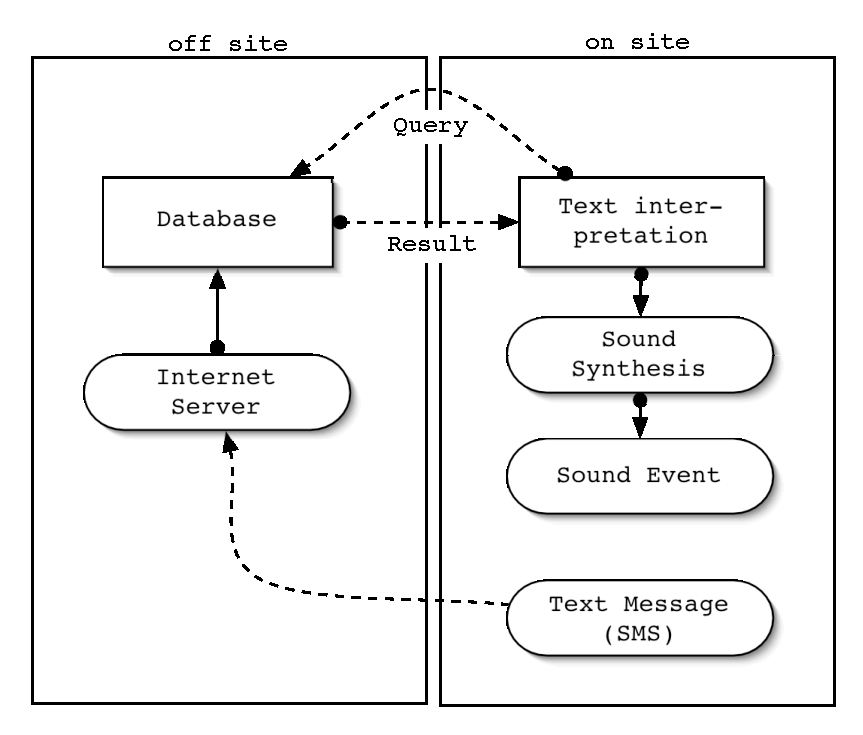
\includegraphics[width=0.7\textwidth]{img/FriskF2}
%     \caption{Diagram of the system for receiving and processing incoming SMS messages.} \label{comm}
%   \end{center}
% \end{figure}

In this work the mobile phone is the interface to the sound production
and to the distribution of sound events. The way the mobile phone is
used here, as a text only input interface, is rather limited and much
of the rest of this article evaluates the advantages the mobile phone
has, despite its limitations as a text input interface. If the only
purpose of etherSound was to allow users to input text that would be
transformed into sound, installing a computer with a keyboard that
would allow visitors to post messages on site would conceivably be
technically less complicated. Another solution, more dynamic than the
one we chose, would have been to implement a voice interface that
allowed for true real time interaction similar to that of the Auracle
project \footcite{auracle}. Although this last option was considered, such
a solution would need a technical and finacial framework that was
beyond our scope.

\section{Communication, time and creativity}
It has been suggested that young people's (specifically teenagers) use
of text messages (SMS), call-credit and mobile phones themselves can
be interpreted as a form of \emph{gifting}: `We will contend that
these gifts are exchanged in performances that have specific meaning
in young people's daily lives and are played out with the intent to
cement social relationships'\footcites[][]{taylor}[See also][]{marcel}.
In other words, text messages have a meaning to the sender and the
recipient that transcends the actual content or meaning of the
message. This is, in more than one way, in accordance with how the
messages sent to \emph{etherSound} were used. The content of the
message as such is not transparent in the resulting sound object, only
the general outline of it (the length, the composition, the number of
syllables, etc.) and every message is `rewarded' with sound; the gift
is always returned. To further develop the meaning of the returning of
the `gift' the temporal aspect of etherSound needs to be considered.

There are two time frames at play in etherSound which bear immediate
significance to this question and they are described here borrowing
terms from Curtis Roads table of temporal hierarchies in music
\footcite[3]{roads}: (1) The `meso time scale' which constitutes the
single message and the resulting sonic events. The mapping between the
message and the sound is linear and relatively consequent. (2) The
`macro time scale' which is the time from when the installation was
started to when it ends. It is within the meso time scale that the
relation between the object and the participant is established and it
is in the dynamics between the meso and the macro time scale that the
`returning of the gift' has curtial significance. It constitutes a
receipt of the contribution; a sonic confirmation that the message has
been received. This kind of immediate response is important in order
to avoid a sensation of exploitation in the participant: Their time,
energy and, in the case of sending text messages from mobile phones,
their money, is not used to fulfill our own opaque objectives hidden
to the participant, but results in a palpable response with a value of
its own. This is the main reason a clear causality between input and
output in the meso time scale is aimed for. Therefore, some effort has
been invested in making each sound object a closed form musical
composition in its own right. However, as soon as the sound object
begins to play back it transmutes into a player in the macro time
scale, in which there is no preconceived musical form but where the
indeterminacy of collective efforts are the main factor. It should be
noted that the relation between the closed form of the meso time scale
and the indeterminacy of the macro time scale is not unproblematic. An
interactive, ongoing and indeterminate, musical creation will
inevitably dismantle the traditional idea of musical form. There is
nothing new with the ``permanent event'' \footcite{barbosa} or the
infinite musical form but it is the effect the indeterminate form has
on the \emph{understanding} and \emph{interpretation}\footnote{Perhaps
  \emph{reading} would be a better word to avoid confusion with the
  musical term interpretation.} of the work from the point of the
participant, and whether the closed form of the message compositions
enhance or degenerate this effect, that is of interest. Will a random
collection of message compositions, each one with a sense of musical
form, generate a large scale (closed) form or will they result in
something else, conceptually different from musical form? I believe
both is possible and, in this particular case, they are both part of
the very core of the artistic intent. It is a question of
perspectives. By opening up the form, the listening experience is
likewise opened up and a multiplicity of perceptive perspectives
becomes possible. However, the most plausible interpretation regarding
the form of \emph{etherSound} is that it is indeed a closed musical
form, but in which the structure of the sounds is open and subject to
change. 


In the age of mass information, consumerist ideology and market
segmentation strategies, individuality is at stake. Laura Martz
asserts that `the \index{Spectacle, Society of the}\index{Debord, Guy!Spectacle}spectacle\footnote{Martz uses the term `the
  specatacle' with a reference to what Guy Debord and the
  situationists called `the society of the \index{Spectacle, Society of the}\index{Debord, Guy!Spectacle}spectacle'
  which includes commodities, art-as-commodity, the mass media and the
  entertainment industry. \cite[See also][]{debord56}} steals every experience and sell it back
to us, but only symbolically'\footcite{martz}, but we believe it is fair to
assume that the desire for personal and individual expression among
the general public and the wish to exercise influence has not
vanished. As we will discuss later, individuality taken too far can be
a problem in the context of an interactive collaborative work such as
the one discussed here, but it is also an asset. Along with curiousity
it is an incitement for wanting to participate, provided that the
action invested results in a perceivable stimuli.

The clear causal relation between the action invested and the sounding
result is a way of giving the participant an experience of involvment
that ultimately could lead to a wish to further explore the causality
of input and output, and give a sensation of understanding. The
suggestion by Taylor et al. that mobile phone originated text
messaging is already used in some circles for \index{interaction!social}social interaction
indicates that the mobile phone is indeed well suited as an interface
for interactive art work where the creativity of the participant is
the object.

\section{Technology, communication and understanding}
Concerning the ideology of the broadening of the audience, Mary J.
Jacob ponders that public participation in the public art of the 90's
never widened the audience \footcite{jacob}. Her contemplation hits a
point, but in order to evaluate the processes in play in our project
we need to consider the social dynamics of new communications
technology. As has already been stated, mobile communication is no
longer a luxuary reserved for the privileged classes, but accessible
to most citizens in the Western World. It may be proposed that luxuary
today is to \emph{not} be accesible, a luxuary that only the secure,
upper classes can afford.

About ten years ago, in the early ages of email communication it was
seen that the nature of the medium had effects on group dynamics:
\begin{squote}
  Advances in computing and telecommunications technology are changing
  how people can meet and make group decisions. Technological changes
  help people cross physical, social, and psychological boundaries and
  have secondary effects on group behavior and decision making.
  Experiments show that compared with face-to-face meeting, a
  computer-mediated discussion leads to; delays; more explicit and
  outspoken advocacy; "flaming"; more equal participation among group
  members; and more extreme, unconventional, or risky decisions.
  \footcite{kiesler92}
\end{squote}
Whether this is also true for SMS communication is a matter of
speculation but it suggests that the means of communication has far
stretching consequences that needs to be considered when designing
interactive interfaces for public art.

We believe that advanced technology, designed for the consumer market,
such as the cellular phone, leans itself well to the purpose of public
interaction and may also help to counteract the tendency for art to
turn itself to the already initiated. What Walter Benjamin
\footcite{benjamin} calls the `advent of mechanical reproduction of art'
has, according to DiMaggio et al., along with other things, `resulted
in a tendency for culture interests to diffuse across class lines'
\footcite{dimaggio}. Benjamin writes:
\begin{squote}
  Around 1900 technical reproduction had reached a standard that not
  only permitted it to reproduce all transmitted works of art and thus
  to cause the most profound change in their impact upon the public;
  it also had captured a place of its own among the artistic
  processes. \footcite[][chap. 1]{benjamin}
\end{squote}
What will be the impact upon the public of the new tools of
distribution of text, audio and images and what will be the role of
the present day technological devices used for communication within
the spheres of creativity and art production? It may not be possible
to answer these questions for many years, but we feel it is of great
interest to evaluate and experiment with the use of these tools within
the realm of artistic and creative expressions.

It may be presumed that consumer market technology, for economical
reasons, is designed to be accessible to as many people as possible
within the target segments assigned by the production companies. The
vast popularity of the mobile phone, despite its technological level
of complexity, coupled with the recent price drops of service charges
suggests that, for mobile phones, this is true. However it should also
be noted that certain segments of the western societies (notably
senior citizens) and the development countries, are still locked out
from, and largely ignored by, this communication revolution. This
taken into consideration, the dynamics of mobile phone usage and
accessibility nevertheless seems to be of a different class than that
of traditional culture consumption. If this holds true, constructing
an interactive interface to an art work based on the use of mobile
phones can potentially open the work to not already initiated groups
of the public.

\section{Creative production and space}
Even though \emph{etherSound} is not site specific in the traditional
sense, it may still be regarded as such since it follows the logic of
the flattened non-space of telecommunication. The phone is tied to a
\index{virtual}virtual space and \emph{etherSound} exists within this space as it is
delimited by the group of people interacting with the installation at
the very moment interaction takes place.  As a result, the context is
\emph{not} the gallery space, but the curatorial idea that delineates
\emph{The Invisible Landscapes}.

\begin{wrapfigure}{r}{0.6\linewidth}
\begin{center}
\includegraphics[width=\linewidth]{img/FriskF1jpg}
\caption{The space at Malm� Konstmuseum where \emph{etherSound} was first realized.}
\end{center}
\end{wrapfigure}
As we have discussed, the emergence of mobile communications, the
Internet and the technological devices that are used to interact on
these networks, has the potential to change the nature of (social)
participation. Now, participation takes place as an extension of
everyday acts. At its best, it does not matter if it is manifested and
glamorized as a single, unique and individual voice. It is not
strained and it is not in a pedagogic mode, but rather follows a mode
of pop culture. It abandons the rational individual and puts emphasis
on the collective in a typical Durkheimian fasion. We could say that
this new form of participation, consisting of clusters of anonymous
random acts, empowers a new structure for creative corporeality which
is never fixed within predetermined conditions but is more reminiscent
of a flow. We want to suggest that it holds potential as a new
coefficient of an autonomous agency of creativity.

The boundary between public and private in mobile phone communication
is not a straight line and can not easily be defined. If we take into
consideration the fact that it is possible to track the location of a
mobile phone, we may even go so far as to say that privacy ceases to
exist the moment ones mobile phone is turned on. But mobile
communication also makes possible a certain kind of private
interaction in the work domain as well as in public spaces. In their
article \footcite{taylor} list a number of circumstances where public
infringes upon private and vice versa. It may be suggested that the
space for mobile communication cannot be distinguished as private
\emph{or} public but creates a new space with its own set of
attributes. Taylor et al. writes:
\begin{squote}
  The phone and its contents, if you like, allows young people to
  differentiate themselves from family or household relations as well
  as cement their own social networks. The phone allows the young
  person to withdraw from the world of the home, for instance, and
  establish a ``micro-world'' through the system of exchange that
  young people employ. \footcite[292]{taylor}
\end{squote}

In \emph{etherSound}, a private act, the composing and sending of a
text message from one's own phone, is transformed to streaming sound
in public. Even though the content of the message remains hidden in
the public sphere, the processes it sets in motion takes place
publicly and may set in motion another private act. What was
originally private, and maybe even meant to stay private, affects the
public space and consequently, the participants share both the
physical and the imaginary, and the two feed off one another.

\section{Authenticity and interpretation}
Active public participation raises a series of questions about
authorship. Who is the composer and who is the performer? Who is the
originator? Who is the commissioner? In \emph{etherSound}, the creator
of the piece can very well be said to be the commissioner, and the
participants, supplying the input, the originators and the curator the
orchestrator. Or, the curator may be perceived as an originator, the
audience as the performers and the creator as the commissioner. We
believe it is impossible and of no use to impose pre-existing roles on
participants. Ultimately, the hybrid role created by different levels
of involvement should be in a state of flow in this work. The
coefficient of plural roles in one individual temporarily appears and
disappears in a subtle and sensitive balance, which, in every
performance will be different. It is `onceness' created by a new
coefficient through SMS participation.

Experience made from presenting \emph{etherSound} at a music
festival\footnote{\emph{Elektrisk Helg}, arranged by Ars Nova, held in
  Malm\"{o}, Sweden in April 2004} is testimony of the difficulty to
achieve this and of the importance of context. Musical performance is
surrounded by old and heavy traditions which implies a rigid
definition of the author. However, since the roles of the players
involved in \emph{etherSound} are interchangeable, confusion arose as
to what the music consisted of, which in turn resulted in some
performers doubting the validity of their participation.

Participating in \emph{etherSound} through SMS is an action started
from an individual initiation at the bottom level, that influences the
whole. The totality will further lead participation on to an
unpredictable outcome. It indicates the power of the situation and the
multitude (not an individual) as factors of creativity. Thus, the
attitude of conviviality naturally directs authenticity of the work in
a more flexible manner. There is no obvious author to credit, and this
opens up for a new form of authenticity, even in relation to
contemporary culture.

As has been noted, the content of a given message was not revealed in
the public sphere except as an abstract series of sonic events and
furthermore, and the audience was not informed of the mapping between
the message and the sound event it generates. This unkown relationship
between the SMS and the sound composition coupled with an expectation
of reflectivity stimulates the imagination of the participant and
navigates them towards a more careful attention to, and translation
of, the sound. This is consistent with Guy Garnett's analysis that:
\begin{squote} [\ldots] music can be roughly considered to be sounds
  made with aesthetic intent, or even sounds listened to with
  aesthetic interest. The former gives more weight to the role of the
  creator, while the latter formulation tends to privilege the
  listener\footcite{Garnett}.
\end{squote}
Hence, content is not only a result of a compositional process, but of
public active participation and in that sense there is nothing to
`understand' in \emph{etherSound} unless you participate. However, if
you do participate, understanding the resulting sound is not dependent
on a thorough insight of the history of art or electronic music
following the idea of the `telematic' piece:
\begin{squote} [\ldots] the observer in an interactive telematic system
  is by definition a participator. In telematic art, meaning is not
  something created by the artist, distributed through the network,
  and \emph{received} by the observer. Meaning is the product of
  interaction between the observer and the system, the content of
  which is in a state of flux, of endless change and transformation
  \footcite{Ascott}.
\end{squote}

\section{Conclusion}
Having discussed the positive effects that portable communication
devices can have in the context of public art it should be mentioned
that this mainly holds true in the Western World. Access to technology
and its uses can easily be taken for granted, but for certain groups,
even in the Western World, it is not self evident how a mobile phone
and all its options are operated, and tangled within this is the
danger of a new kind of class hierarchy based on knowledge of, use of
and access to communications technology.

In this project we have showed that the cellular phone, and its
owners' ability to send text messages from it, can successfully be
used as an interface for public interaction. We also believe that,
given our intentions, the SMS interface has some advantages compared
to other possible solutions. From a practical angle it is widespread,
comparatively simple to use, it is private and it is surrounded with a
large framework that makes it easy to integrate it in an artistic
work. In addition, in the Western World, it has already coalesced into
our private and professional lives and has become a tool for \index{interaction!social}social interaction. Participation can per se open up the work to groups of
people not familiar with contemporary sound art and an interactive
interface built around the mobile phone may contribute to in some
degree neutralizing the class hierarchies in arts consumption.

Even though interaction with \emph{etherSound} stems from an
individual wish to participate, the interface and the system center on
the public rather than the private. This transformation from private
to public opens up for a new sensation of space and an auspicious and
dynamic impression of creativity. Moreover we have suggested that
communication itself is a corresponding form of creativity.

A thought that was never implemented due to lack of funds and
technical equipment, was to, in addition to the location specific
installation, stream the sound on the Internet. This would allow for
groups of people that, for various reasons, did not have access to the
location of the exhibition hall, to participate and it would greatly
expand the accessibility. Further, it would be interesting to try to
allow for greater depth in the system and yield for `expert'
performance. This would however have to be done with great care in
order not to loose the collective focus.

%%% Local Variables: 
%%% mode: latex
%%% TeX-master: "../stim_create"
%%% End: 


\chapter*{\bibname}

\bibliography{bibliography}
\bibliographystyle{newapa}

\end{document}
%%% Local Variables: 
%%% mode: latex
%%% TeX-master: t
%%% End: 
